\begin{frame}
    \frametitle{Bài toán khởi động}
    \begin{columns}
        \begin{column}{0.5\textwidth}
            \vspace{-16pt}

            \begin{figure}
                \centering
                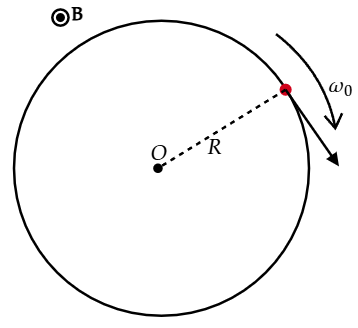
\includegraphics[width=3.5cm, height=3.5cm]{Content/Figure/initial_motion.png}   
                \caption{Chuyển động ban đầu}
            \end{figure}
            \begin{itemize}
                \item  \(\mathbf{B}=\frac{B_0}{r^n}\hat{z}\).
                \item \(\omega_0 =\frac{eB_0}{mR^n}\).
            \end{itemize}
           
        \end{column}
        \begin{column}{0.5\textwidth}
            \vspace{-2pt}

            \begin{figure}
                \centering
                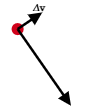
\includegraphics[width=2cm, height=3cm]{Content/Figure/initial_motion2.png}
                \caption{Nhiễu động nhỏ}
            \end{figure}
            \begin{itemize}
                \item \(\lvert\Delta\mathbf{v}\rvert \ll\omega_0 R\).
                \item \(r_{\text{max}}=R+\delta,\quad \delta\ll R\).
            \end{itemize}
        \end{column}
    \end{columns}
\end{frame}
\begin{frame}
    \frametitle{Lời giải}
    Từ định luật II Newton và định luật Lorentz: \[m\mathbf{a}=e\mathbf{v}\times\mathbf{B}.\]
    Kết quả thu được: 
    \begin{equation}\label{eq1}
    \mathbf{a}=\begin{bmatrix}
        \ddot{r}-r\dot{\phi}^2\\
        r\ddot{\phi}+2\dot{r}\dot{\phi}\\
        \ddot{z}
    \end{bmatrix}=\frac{eB_0}{m}\begin{bmatrix}
        r^{1-n}\dot\phi\\
        -r^{-n}\dot{r}\\
        0
    \end{bmatrix}.
    \end{equation}
\end{frame}
\begin{frame}
    \frametitle{Lời giải}
    Chú ý rằng, \[r\ddot{\phi}+2\dot{r}\dot{\phi}=\frac{1}{r}\frac{d}{dt}(r^2 \dot\phi).\]
    Kết hợp với phương trình~\eqref{eq1}, và thu được
    \[\frac{d}{dt}\left(r^2\dot\phi +\frac{1}{2-n}\frac{eB_0}{m}r^{2-n}\right)=0.\]
    Hay, \[r^2\dot\phi +\frac{1}{2-n}\frac{eB_0}{m}r^{2-n}=const.~~(!)\]
    Kết quả cuối cùng: \begin{equation}
        r=R+\delta\cos\left(\omega_0\sqrt{1-n} t+\frac{\pi}{2}\right).
    \end{equation}
\end{frame}
